\label{tutorial:ajpf:troubleshooting}

This is the second in a series of tutorials on the use of the \ajpf\ model checking program.  This tutorial covers \jpf\ configuration\index{configuration!JPF}\index{JPF!configuration}\index{JPF} files in more detail as well as techniques for troubleshooting model checking\index{model checking}.

Files for this tutorial can be found in the \texttt{mcapl} distribution in the directory 
\begin{quote}
\texttt{src/examples/gwendolen/ajpf\_tutorials/tutorial2}.
\end{quote}

The tutorials assume some familiarity with the basics of running Java programs either at the command line or in Eclipse and some familiarity with the syntax and semantics of Linear Temporal Logic, and the use of B\"{u}chi Automata in model checking.

\section{\jpf\ Configuration Files}
As mentioned \intutorial{\ajpf}{1}{tutorial:ajpf:psl}, \jpf\ had an extensive set of configuration options which you can find in the JPF documentation~\footnote{Currently to be found at \url{http://babelfish.arc.nasa.gov/trac/jpf}}. We only examined the most basic \intutorial{\ajpf}{1}{tutorial:ajpf:psl}  but in this tutorial we will cover a few more that are useful, particularly when debugging\index{debugging!program} a program you are attempting to model check.

\begin{sloppypar}
In the tutorial directory you will find a simple \gwendolen\ program, \texttt{twopickupagents.gwen}\index{example!twopickupagents}.  This contains two agents, one holding a block and one holding a flag.  Each agent puts down what they are holding.  If the agent with the block puts it down before the agent with the flag puts the flag down, then the agent with the flag will pick up the box.  The agent with the flag also performs an action with random consequences after it puts down the flag.
\end{sloppypar}

\subsection{TwoPickUpAgents\_basic.jpf}\index{example!twopickupagents} \texttt{TwoPickUpAgents\_basic.jpf} is a minimal configuration file containing only options discussed \intutorial{\ajpf}{1}{tutorial:ajpf:psl}.  This generates the following output:

\begin{verbatim}
JavaPathfinder core system v8.0 (rev ${version}) - (C) 2005-2014 United States Government. All rights reserved.


====================================================== system under test
ail.util.AJPF_w_AIL.main("/Users/louiseadennis/Eclipse/mcapl/src/examples/gwendolen/ajpf_tutorials/tutorial2/TwoPickUpAgents.ail","/Users/louiseadennis/Eclipse/mcapl/src/examples/gwendolen/ajpf_tutorials/tutorial2/PickUpAgent.psl","1")

====================================================== search started: 27/02/15 16:59

====================================================== results
no errors detected

====================================================== statistics
elapsed time:       00:00:03
states:             new=13,visited=10,backtracked=23,end=0
search:             maxDepth=5,constraints=0
choice generators:  thread=1 (signal=0,lock=1,sharedRef=0,threadApi=0,reschedule=0), data=13
heap:               new=84557,released=80981,maxLive=3504,gcCycles=23
instructions:       7938974
max memory:         309MB
loaded code:        classes=309,methods=4795

====================================================== search finished: 27/02/15 16:59
\end{verbatim}

This is obviously fine as output in situations where the model checking completes quickly and with \texttt{no errors detected} but gives the user very little to go on if there is a problem or the model checking is taking a long time and they are not sure whether to kill the attempt or not.

\subsection{TwoPickUpAgents\_ExecTracker.jpf}\index{example!twopickupagents}

\texttt{TwoPickUpAgents\_ExecTracker.jpf} adds the configuration option:

\begin{verbatim}
listener+=,.listener.ExecTracker
et.print_insn=false
et.show_shared=false
\end{verbatim}\index{JPF!configuration!listener}\index{et.print\_insn}\index{et.show\_shared}

Adding \texttt{listener.ExecTracker} to \jpf's listeners\index{JPF!listener} means that it collects more information about progress as it goes and then prints this information out.  The next two lines suppress some of this information which is generally less useful in \ajpf.  With these settings the following output is generated (only the start is shown):

\begin{small}
\begin{verbatim}
		 # choice: gov.nasa.jpf.vm.choice.ThreadChoiceFromSet {id:"ROOT" ,1/1,isCascaded:false}
		 # garbage collection
----------------------------------- [1] forward: 0 new
		 # choice: gov.nasa.jpf.vm.choice.IntChoiceFromSet[id="probabilisticChoice",isCascaded:false,>0,1]
		 # garbage collection
----------------------------------- [2] forward: 1 new
		 # choice: gov.nasa.jpf.vm.choice.IntChoiceFromSet[id="probabilisticChoice",isCascaded:false,>0,1]
		 # garbage collection
----------------------------------- [3] forward: 2 new
		 # choice: gov.nasa.jpf.vm.choice.IntChoiceFromSet[id="probabilisticChoice",isCascaded:false,>0,1]
		 # garbage collection
----------------------------------- [4] forward: 3 new
		 # choice: gov.nasa.jpf.vm.choice.IntChoiceFromSet[id="probabilisticChoice",isCascaded:false,>0,1]
		 # garbage collection
----------------------------------- [5] forward: 4 new
		 # choice: gov.nasa.jpf.vm.choice.IntChoiceFromSet[id="probabilisticChoice",isCascaded:false,>0,1]
		 # garbage collection
----------------------------------- [6] forward: 5 new
		 # choice: gov.nasa.jpf.vm.choice.IntChoiceFromSet[id="probabilisticChoice",isCascaded:false,>0,1]
		 # garbage collection
----------------------------------- [7] forward: 6 visited
----------------------------------- [6] backtrack: 5
		 # choice: gov.nasa.jpf.vm.choice.IntChoiceFromSet[id="probabilisticChoice",isCascaded:false,0,>1]
		 # garbage collection
----------------------------------- [7] forward: 7 visited
----------------------------------- [6] backtrack: 5
----------------------------------- [6] done: 5
----------------------------------- [5] backtrack: 4
		 # choice: gov.nasa.jpf.vm.choice.IntChoiceFromSet[id="probabilisticChoice",isCascaded:false,0,>1]
		 # garbage collection
----------------------------------- [6] forward: 8 new
		 # choice: gov.nasa.jpf.vm.choice.IntChoiceFromSet[id="probabilisticChoice",isCascaded:false,>0,1]
		 # garbage collection
----------------------------------- [7] forward: 6 visited
----------------------------------- [6] backtrack: 8
\end{verbatim}
\end{small}

Every time \jpf\ generates a new state\index{JPF!model state} for model checking\index{model checking} it assigns that state a number.  In the output here you can see it generating new states 0 through to 7 and advancing forward to each state.  You then see it backtracking back to state 5 (which is fully explored \texttt{done}\index{model checking!branch done}) and then state 4 at which point it finds a branching point in the search space and advances to state 8 and then again to state 6 which it has visited already and so backtracks to 8\index{backtracking}.

Typically search space\index{search space}\index{search space!branching}\index{model!state!generation} branching is caused either whenever a random value is generated\index{probabilisticChoice}.  This happens most often when the multi-agent system scheduler\index{scheduler!effect on model checking} must choose between several agents.

Random value generation activates an \texttt{IntChoiceFromSet}\index{IntChoiceFromSet (class)} choice generator\index{choice generator} (which picks a random integer from a set -- usually picking one number from a range).  The scheduler\index{scheduler} keeps track of the agents which are awake and assigns an integer to them.  Since there are only two agents, there is no choice if one is asleep, but you can see when the choice between \texttt{0} and \texttt{1}.

The numbers in square brackets -- \texttt{[7]}, \texttt{[6]} etc. indicate the depth that model checking\index{model checking!depth}\index{model checking} has reached in the search tree\index{model checking!search tree}\index{search space}.  If these numbers become very large without apparent reason then it may well be the case that the search has encountered an infinite branch of the tree and needs to be killed.

\subsection{Logging}\index{JPF!logging}
\jpf\ suppresses the logging configuration\index{JPF!configuration}\index{configuration!JPF} you have in your \ail\ configuration\index{configuration!AIL}\index{AIL!configuration} files so you need to add any logging configurations you want to the \jpf\ configuration file.  Useful classes when debugging\index{debugging}\index{debugging!model checking failed} a model checking run are

\begin{description}
\item[ail.mas.DefaultEnvironment] At the \texttt{info} level this prints out any actions the agent performs.  Since the scheduler\index{scheduler} normally only switches between agents when one sleeps\index{sleeping} or performs an action\index{action} this can be useful for tracking progress on this model checking branch.\index{DefaultEnvironment (class)}
\item[ajpf.MCAPLAgent]\index{MCAPLAgent (class)} At the \texttt{info} level this prints information when an agent sleeps\index{sleeping} or wakes.  Again this can be useful for seeing what has triggered a scheduler\index{scheduler} switch.  It can also be useful for tracking which agents are awake and so deducing which one is being picked from the set by the \texttt{IntChoiceFromSet}\index{IntChoiceFromSet (class)} choice generator\index{choice generator}.
\item[ajpf.product.Product]\index{Product (class)} At the \texttt{info} level this prints out the current path\index{model checking!search tree!current path} through the search tree\index{model checking!search tree} being explored by the agent.  This can be useful just to get a feel for the agents' progress through the search space.  It can also be useful, when an error is thrown and in conjunction with some combination of logging actions\index{action}, sleeping\index{sleeping} and waking behaviour and (if necessary) internal agent states, to work out why a property has failed to hold.

It also prints the message \texttt{Always True from Now On}\index{Always True from Now On} when exploration of a branch of the search tree\index{model checking!search tree} is halted because the system deduces that the property will be true for the rest of that branch.  This typically occurs when the property is something like $\sometime \phi$ (i.e., $\phi$ will eventually\index{property!eventually} occur) and the search space\index{search space}\index{search space!pruning} is pruned once $\phi$ becomes true.
\item[ajpf.psl.buchi.BuchiAutomaton]\index{BuchiAutomaton (class)} At the \texttt{info} level this prints out the B\"{u}chi Automaton\index{B\"{u}chi Automaton} that has been generated from the the property that is to be proved.  Again this is useful, when model checking\index{model checking} fails, for working out what property was expected to hold in that state.
\item[ail.semantics.AILAgent]\index{AILAgent (class)} At the \texttt{fine} level this prints out the internal agent state\index{agent state} once every reasoning cycle\index{reasoning cycle}.  Be warned that this produces a lot of output in the course of a model checking\index{model checking} run.
\end{description}

\begin{sloppypar}
In general, when working on a program for model checking\index{model checking} it is useful to have the \text{ExecTracker} listener enabled and \texttt{ajpf.MCAPLAgent}\index{MCAPLAgent (class)}, \texttt{ajpf.product.Product}\index{Product (class)} and any environment\index{environment} loggers (so typically \texttt{ail.mas.DefaultEnvironment}\index{DefaultEnvironment (class)} and any sub-classes of that you are using) set at info.   This provides a useful starting point for accessing information about model checking.
\end{sloppypar}

\texttt{TwoPickUpAgents\_Logging.jpf}\index{example!logging}\index{example!twopickupagents} has this set up.  It's output starts

\begin{verbatim}
[INFO] Adding 0 to []
----------------------------------- [1] forward: 0 new
		 # choice: gov.nasa.jpf.vm.choice.IntChoiceFromSet[id="probabilisticChoice",isCascaded:false,>0,1]
[INFO] ag2 done putdown(flag)
		 # garbage collection
[INFO] Adding 1 to [0]
----------------------------------- [2] forward: 1 new
		 # choice: gov.nasa.jpf.vm.choice.IntChoiceFromSet[id="probabilisticChoice",isCascaded:false,>0,1]
		 # garbage collection
[INFO] Adding 2 to [0, 1]
----------------------------------- [3] forward: 2 new
		 # choice: gov.nasa.jpf.vm.choice.IntChoiceFromSet[id="probabilisticChoice",isCascaded:false,>0,1]
[INFO] Block 1 is visible
		 # garbage collection
[INFO] Adding 3 to [0, 1, 2]
----------------------------------- [4] forward: 3 new
		 # choice: gov.nasa.jpf.vm.choice.IntChoiceFromSet[id="probabilisticChoice",isCascaded:false,>0,1]
[INFO] Block 2 is visible
[INFO] ag2 done random
		 # garbage collection
[INFO] Adding 4 to [0, 1, 2, 3]
----------------------------------- [5] forward: 4 new
		 # choice: gov.nasa.jpf.vm.choice.IntChoiceFromSet[id="probabilisticChoice",isCascaded:false,>0,1]
[INFO] Sleeping agent ag2
[INFO] Waking agent ag2
[INFO] ag1 done putdown(block)
		 # garbage collection
[INFO] Adding 5 to [0, 1, 2, 3, 4]
----------------------------------- [6] forward: 5 new
		 # choice: gov.nasa.jpf.vm.choice.IntChoiceFromSet[id="probabilisticChoice",isCascaded:false,>0,1]
[INFO] Sleeping agent ag2
		 # garbage collection
[INFO] Adding 6 to [0, 1, 2, 3, 4, 5, 6]
[INFO] Always True from Now On
----------------------------------- [7] forward: 6 visited
----------------------------------- [6] backtrack: 5
		 # choice: gov.nasa.jpf.vm.choice.IntChoiceFromSet[id="probabilisticChoice",isCascaded:false,0,>1]
[INFO] Sleeping agent ag1
		 # garbage collection
[INFO] Adding 7 to [0, 1, 2, 3, 4, 5, 7]
[INFO] Always True from Now On
----------------------------------- [7] forward: 7 visited
----------------------------------- [6] backtrack: 5
----------------------------------- [6] done: 5
----------------------------------- [5] backtrack: 4
		 # choice: gov.nasa.jpf.vm.choice.IntChoiceFromSet[id="probabilisticChoice",isCascaded:false,0,>1]
[INFO] ag1 done putdown(block)
		 # garbage collection
[INFO] Adding 8 to [0, 1, 2, 3, 4]
----------------------------------- [6] forward: 8 new
		 # choice: gov.nasa.jpf.vm.choice.IntChoiceFromSet[id="probabilisticChoice",isCascaded:false,>0,1]
[INFO] Sleeping agent ag2
		 # garbage collection
[INFO] Adding 6 to [0, 1, 2, 3, 4, 8]
----------------------------------- [7] forward: 6 visited
----------------------------------- [6] backtrack: 8
		 # choice: gov.nasa.jpf.vm.choice.IntChoiceFromSet[id="probabilisticChoice",isCascaded:false,0,>1]
[INFO] Sleeping agent ag1
		 # garbage collection
[INFO] Adding 7 to [0, 1, 2, 3, 4, 8]
----------------------------------- [7] forward: 7 visited
----------------------------------- [6] backtrack: 8
----------------------------------- [6] done: 8
----------------------------------- [5] backtrack: 4
----------------------------------- [5] done: 4
----------------------------------- [4] backtrack: 3
		 # choice: gov.nasa.jpf.vm.choice.IntChoiceFromSet[id="probabilisticChoice",isCascaded:false,0,>1]
[INFO] Block 2 is not visible
[INFO] ag2 done random
		 # garbage collection
[INFO] Adding 9 to [0, 1, 2, 3]
----------------------------------- [5] forward: 9 new
		 # choice: gov.nasa.jpf.vm.choice.IntChoiceFromSet[id="probabilisticChoice",isCascaded:false,>0,1]
[INFO] Sleeping agent ag2
[INFO] Waking agent ag2
[INFO] ag1 done putdown(block)
		 # garbage collection
[INFO] Adding 10 to [0, 1, 2, 3, 9]
----------------------------------- [6] forward: 10 new
\end{verbatim}
You can see the additional information provided by the loggers here, in terms of printing out the current path through the search tree\index{model checking}\index{model checking!search tree}, reporting on sleeping\index{sleeping} and waking behaviour, etc.,

{\bf Important Note:} While the additional output information can be very useful for understanding what is happening during a model checking run, printing output slows down the computation.  If speed of model checking\index{model checking!speed} is important then it is best to turn off all logging and the \texttt{ExecTracker}.

\subsection{Saving the log to a file}
It is possible to save log message\index{model checking!log file} generated by the \ail\ to a file by including \texttt{log.output = filename} (where \texttt{filename} is the name of the file you want to use) in your JPF configuration\index{configuration!JPF}\index{JPF!configuration} file.  Unfortunately this does not save the output of the \texttt{ExecTracker} to the file but may nevertheless be useful.

\section{What to do when Model Checking Fails}\index{model checking}\index{model checking!failure}

\begin{sloppypar}
\texttt{TwoPickUpAgents\_FalseProp.jpf}\index{example!twopickupagents} attempts to prove the property $\sometime \lbelief{ag2}{hold(block)}$ which isn't true.  The configuration file uses the normal loggers but doesn't have the \texttt{ExecTracker} listener\footnote{Largely to keep the output compact.}.  The following output is generated.
\end{sloppypar}

\begin{footnotesize}
\begin{verbatim}
====================================================== system under test
ail.util.AJPF_w_AIL.main("/Users/lad/Eclipse/mcapl/src/examples/gwendolen/ajpf_tutorials/tutorial2/TwoPickUpAgents.ail","/Users/lad/Eclipse/mcapl/src/examples/gwendolen/ajpf_tutorials/tutorial2/PickUpAgent.psl","2")

====================================================== search started: 28/04/17 15:58
[INFO] Adding 0 to []
[INFO] ag2 done putdown(flag)
[INFO] Adding 1 to [0]
[INFO] Adding 2 to [0, 1]
[INFO] Block 1 is visible
[INFO] Adding 3 to [0, 1, 2]
[INFO] Block 2 is visible
[INFO] ag2 done random
[INFO] Adding 4 to [0, 1, 2, 3]
[INFO] Sleeping agent ag2
[INFO] Waking agent ag2
[INFO] ag1 done putdown(block)
[INFO] Adding 5 to [0, 1, 2, 3, 4]
[INFO] Sleeping agent ag2
[INFO] Adding 6 to [0, 1, 2, 3, 4, 5]

====================================================== error 1
ajpf.MCAPLListener
An Accepting Path has been found: 
[MS: 0, BS: 2, UN: 0], [MS: 1, BS: 2, UN: 0], [MS: 2, BS: 2, UN: 0], [MS: 3, BS: 2, UN: 0], [MS: 4, BS: 2, UN: 0],
[MS: 5, BS: 2, UN: 0], [MS: 6, BS: 2, UN: 0], 

====================================================== snapshot #1
no live threads

====================================================== results
error #1: ajpf.MCAPLListener "An Accepting Path has been found:  [MS: 0, BS: 2, ..."
\end{verbatim}
\end{footnotesize}

As can be seen at the end of the failed run this prints out the accepting path\index{accepting path} that it has found that makes the property false.  This path is a sequence of triples consisting of the state in the model\index{model!state}, \texttt{MS}, the state in the B\"{u}chi automaton\index{B\"{u}chi Automaton}\index{B\"{u}chi Automaton!state} generated from the negation of the property, \texttt{BS}, and lastly a count of the number of until statements\index{until statements} that have been passed in this branch/loop of the search space (This counter is explained in~\cite{Gerth:1995:SOA:645837.670574} -- it isn't normally useful for debugging\index{debugging!properties} properties but is included for completeness).

So we can see that the accepting path\index{accepting path} through the model\index{model} is 0,1,2,3,4,5,6 and we can work out what happens on that path from the logging output: ag2 puts down the flag, both blocks becomes visible, ag2 does random and then sleeps, ag1 puts down the block, waking ag2 which then sleeps again.  All these states in the model are paired with state 2 in the B\"{u}chi Automaton\index{model!state}\index{B\"{u}chi Automaton!state}.  To see the B\"{u}chi Automaton you have to add \texttt{ajpf.psl.buchi.BuchiAutomaton}\index{BuchiAutomaton (class)} to the logging.

If you do this you get the following print out at the start:

\begin{verbatim}
[INFO] Number: 2
Incoming States: 0,2,
True in this State: ~B(ag2,hold(block())),~T R ~B(ag2,hold(block())),
True in next State: ~T R ~B(ag2,hold(block())),
\end{verbatim}

The property has created a very simple B\"{u}chi Automaton\index{B\"{u}chi Automaton}.  It has been given the number 2 in the automaton generation process.  It has two incoming states 0 (which is the start state) and 2 (i.e., itself).  It has two properties that hold in that state $\neg \lbelief{ag2}{hold(block)}$ (ag2 doesn't believe it is holding the block) and $\neg \top {\cal R} \neg \lbelief{ag2}{hold(block)}$ (false ($\neg \top$) released by ag2 doesn't believe it is holding the block -- which under standard LTL transformations means $\always \neg \lbelief{ag2}{hold(block)}$ (it is always the case that ag2 doesn't believe it is holding the block)).  In the next state this should also hold.  For debugging\index{debugging}\index{debugging!model checking failed} failed model checking runs it is normally safe to ignore the properties that should hold in the next state, and any temporal properties that should hold in the current state, so this automaton can be visualised as in figure~\ref{fig:automaton}.

\begin{figure}[htb]
\begin{center}
%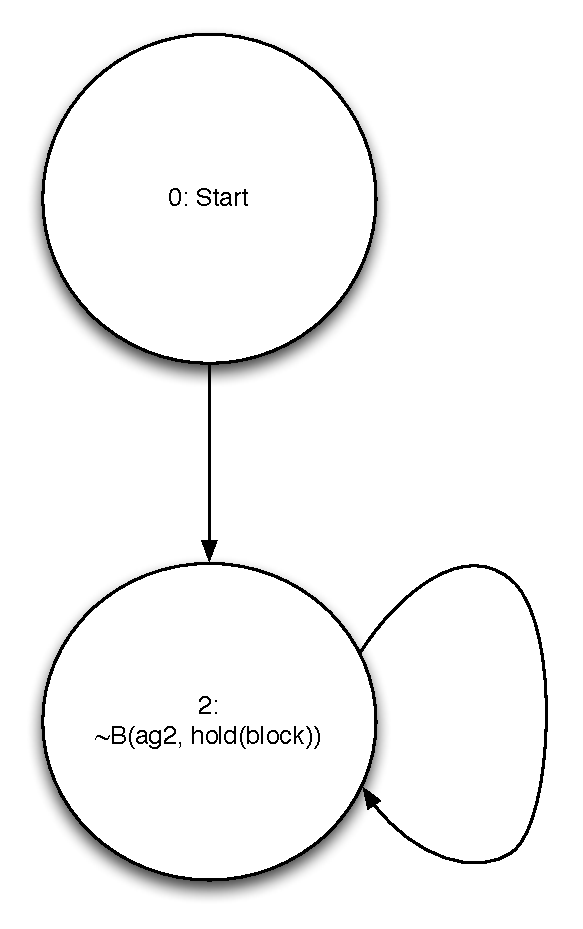
\includegraphics[width=2in]{images/property_automata.pdf}
\end{center}
\caption{The Property Automaton\index{B\"{u}chi Automaton} for $\neg \sometime \lbelief{ag2}{hold(block)}$}
\label{fig:automaton}
\end{figure}

I.e. a single state automaton\index{B\"{u}chi Automaton} in which $\lbelief{ag2}{hold(block)}$ is never true.  The model checking has failed because this state is true for every state in the model along the path 0,1,2,3,4,5,6 (you can look in the program to se why).

\section{Replaying a Counter-example}
When model-checking fails the branch it has failed on has essentially generated a counter-example for the property.  Sometimes you will want to replay this counter-example\index{replay model branch} in the \ail\ without performing model-checking.  \ajpf\ has \emph{record}\index{record model checking} and \emph{replay} functionality to assist with this.

To obtain a record\index{record model checking} of a model checking\index{model checking} run you will need to set \emph{logging mode} in the \emph{\ail\ configuration file}\index{configuration!AIL}\index{AIL!configuration} (using \texttt{ajpf.record = true})\index{ajpf.record} and then set the the logging level to fine in \texttt{ajpf.util.choice.ChoiceRecord})\index{ChoiceRecord (class)}.

\texttt{TwoPickupAgents\_Recording.txt} has this setup.  Its output starts:
\begin{verbatim}
		 # choice: gov.nasa.jpf.vm.choice.ThreadChoiceFromSet {id:"ROOT" ,1/1,isCascaded:false}
		 # garbage collection
----------------------------------- [1] forward: 0 new
		 # choice: gov.nasa.jpf.vm.choice.IntChoiceFromSet[id="probabilisticChoice",isCascaded:false,>0,1]
[FINE] Record: [0]
[FINE] Record: [0, 0]
		 # garbage collection
----------------------------------- [2] forward: 1 new
		 # choice: gov.nasa.jpf.vm.choice.IntChoiceFromSet[id="probabilisticChoice",isCascaded:false,>0,1]
[FINE] Record: [0, 0, 0]
[FINE] Record: [0, 0, 0, 0]
		 # garbage collection
----------------------------------- [3] forward: 2 new
		 # choice: gov.nasa.jpf.vm.choice.IntChoiceFromSet[id="probabilisticChoice",isCascaded:false,>0,1]
[FINE] Record: [0, 0, 0, 0, 0]
		 # garbage collection
----------------------------------- [4] forward: 3 new
		 # choice: gov.nasa.jpf.vm.choice.IntChoiceFromSet[id="probabilisticChoice",isCascaded:false,>0,1]
[FINE] Record: [0, 0, 0, 0, 0, 0]
		 # garbage collection
----------------------------------- [5] forward: 4 new
		 # choice: gov.nasa.jpf.vm.choice.IntChoiceFromSet[id="probabilisticChoice",isCascaded:false,>0,1]
[FINE] Record: [0, 0, 0, 0, 0, 0, 0]
[FINE] Record: [0, 0, 0, 0, 0, 0, 0, 0]
[FINE] Record: [0, 0, 0, 0, 0, 0, 0, 0, 0]
[FINE] Record: [0, 0, 0, 0, 0, 0, 0, 0, 0, 0]
		 # garbage collection
----------------------------------- [6] forward: 5 new
		 # choice: gov.nasa.jpf.vm.choice.IntChoiceFromSet[id="probabilisticChoice",isCascaded:false,>0,1]
[FINE] Record: [0, 0, 0, 0, 0, 0, 0, 0, 0, 0, 0]
[FINE] Record: [0, 0, 0, 0, 0, 0, 0, 0, 0, 0, 0, 0]
[FINE] Record: [0, 0, 0, 0, 0, 0, 0, 0, 0, 0, 0, 0, 0]
[FINE] Record: [0, 0, 0, 0, 0, 0, 0, 0, 0, 0, 0, 0, 0, 0]
		 # garbage collection
----------------------------------- [7] forward: 6 visited
----------------------------------- [6] backtrack: 5
		 # choice: gov.nasa.jpf.vm.choice.IntChoiceFromSet[id="probabilisticChoice",isCascaded:false,0,>1]
[FINE] Record: [0, 0, 0, 0, 0, 0, 0, 0, 0, 0, 1]
[FINE] Record: [0, 0, 0, 0, 0, 0, 0, 0, 0, 0, 1, 1]
[FINE] Record: [0, 0, 0, 0, 0, 0, 0, 0, 0, 0, 1, 1, 0]
[FINE] Record: [0, 0, 0, 0, 0, 0, 0, 0, 0, 0, 1, 1, 0, 0]
		 # garbage collection
\end{verbatim}
The lines starting \texttt{[FINE] Record:} show the record\index{record model checking} of choices at that point.  To replay\index{replay model branch} a particular branch through the search tree in \ail\ without model checking do the following:
\begin{enumerate}
\item Paste the relevant record list, e.g. \texttt{[0, 0, 0, 0, 0, 0, 0, 0, 0, 0, 1]} into the file \texttt{record.txt} in the \texttt{records} directory of the \mcapl\ distribution.
\item Replace the line \texttt{ajpf.record = true}\index{ajpf.record} in your \ail\ configuration\index{configuration!AIL}\index{AIL!configuration} file with the line \texttt{ajpf.replay = true}\index{ajpf.replay}.  
\item Run the program in \ail\ as normal.
\end{enumerate}

If you want to use a different file to \texttt{record.txt} to store the record for replay you can, but you will need to set \texttt{ajpf.replay.file}\index{ajpf.replay.file} in the \ail\ configuration\index{configuration!AIL}\index{AIL!configuration} file appropriate in order to replay that record.

{\bf (Use of Random) Please note:} that it is important for record and replay to work correctly that all choice points in the program are used in the record.  Among other things this means that Java's \texttt{Random}\index{Random (class)} class {\bf can not} be used in constructing environments and \ajpf's \texttt{Choice}\index{Choice (class)} class should be used instead.  

\section{Forcing Transitions in the Agent's Reasoning Cycle}
In the examples considered so far in this tutorial, \ajpf{} has only generated new states for the model\index{model!state!generation} when \jpf{} would generate a state.  This has been when there has been a scheduling choice between the two agents.  While this is often sufficient for many model checking\index{model checking} problems it does mean that the property is only checked when the agent program has done significant processing.  This means that states of interest can sometimes be ommitted for checking -- particularly in the case of the ($\lintendtodo{\AILagent}{f}$\index{$\lintendtodofunc$}\index{property!intending to do} properties where you are interested in whether the agent ever has an intention that contains a particular action, the action may well have been removed from the intention before the property is checked).

\begin{sloppypar}
By default, in fact, \ajpf{} generates a new model state\index{model!state!generation} every time the agent advances its reasoning cycle\index{reasoning cycle}.  \texttt{TwoPickUpAgents\_EveryTransition.jpf}\index{example!twopickupagents} runs the above examples in this mode.  If you run it you will notice that there are a lot more states in the model and that most of them are generated by a \texttt{NewAgentProgramState}\index{NewAgentProgramState} choice generator that doesn't actually cause any branching.  This behaviour can be switched off by including \texttt{ajpf.transition\_every\_reasoning\_cycle = false}\index{ajpf.transition\_every\_reasoning\_cycle} in the \ail{} configuration\index{configuration!AIL}\index{AIL!configuration} file (Note this has to be the \emph{AIL configuration file} not the \emph{JPF configuration file}\index{configuration!JPF}\index{JPF!configuration}).
\end{sloppypar}


